\documentclass[11pt]{article}

\usepackage{amsmath}
\usepackage{graphicx}
\usepackage{booktabs}
\usepackage[backend=biber,style=authoryear]{biblatex}
\addbibresource{refs.bib}

% Visual angle in degrees, used throughout.
\newcommand{\vdeg}[1]{\ensuremath{#1^{\circ}}}

\title{Fixational Eye Movements Shape Early Visual Responses}
\author{Ada Example \and Grace Sample}
\date{November 2026}

\begin{document}

\maketitle

\begin{abstract}
Small eye movements persist during fixation and shift the retinal image by
many photoreceptor widths. We measured how these movements change the
responses of neurons in the lateral geniculate nucleus. Responses were
\emph{larger} after a microsaccade than before it, and the effect grew with
stimulus contrast.
\end{abstract}

\section{Introduction}
\label{sec:intro}

The eyes are never still. Even during steady fixation they drift and make
small, rapid jumps called \emph{microsaccades} \parencite{rolfs2009}. These
movements matter for perception: \textcite{rucci2015} argue that they
\textbf{reformat} the visual input rather than blur it. An earlier account
\cite{missing2019} reached the opposite conclusion, which we revisit in
Section~\ref{sec:results}.

We address three questions:
\begin{itemize}
  \item Do responses change around the time of a microsaccade?
  \item Does the change depend on stimulus contrast?
  \item Is the change explained by the shift of the retinal image alone?
\end{itemize}

Stimuli subtended \vdeg{0.5} and were shown at 60\% contrast. The gain
$g = R_{\text{post}} / R_{\text{pre}}$ summarizes the effect for each neuron.

\section{Methods}
\label{sec:methods}

\subsection{Eye tracking}

Eye position was sampled at 1~kHz. Microsaccades were detected with a
velocity threshold, following \textcite{engbert2003}. A movement counted as
a microsaccade when its amplitude was below \vdeg{1}.

\subsection{Analysis}

For each neuron we counted spikes in two windows of width $w = 100$~ms.
The firing rate in a window is
\[
  R = \frac{1}{N w} \sum_{i=1}^{N} k_i ,
\]
where $k_i$ is the spike count on trial $i$ and $N$ is the number of trials.

We recorded \NumNeurons{} neurons over \NumSessions\ sessions. The gain
$\Gain$ had a 95\% interval of \GainCI, and $n = \NumNeurons$ throughout.


\section{Results}
\label{sec:results}

Figure~\ref{fig:trace} shows the mean eye position around a microsaccade.
Responses rose within 50~ms of the movement, as summarized in
Table~\ref{tab:gain}. The appendix that would hold the control analysis is
not written yet (Section~\ref{sec:missing}).

\begin{figure}[ht]
  \centering
  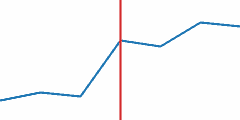
\includegraphics[width=0.6\linewidth]{figures/trace.png}
  \caption{Mean horizontal eye position aligned to microsaccade onset
  (red line).}
  \label{fig:trace}
\end{figure}

\begin{table}[ht]
  \centering
  \caption{Response gain by stimulus contrast.}
  \label{tab:gain}
  \begin{tabular}{lcc}
    \toprule
    Contrast & Neurons & Gain \\
    \midrule
    Low & 24 & 1.08 \\
    Medium & 31 & 1.21 \\
    High & 28 & 1.37 \\
    \bottomrule
  \end{tabular}
\end{table}

The gain followed a saturating function of contrast $c$,
\begin{equation}
  g(c) = 1 + g_{\max} \frac{c^{n}}{c^{n} + c_{50}^{n}},
  \label{eq:gain}
\end{equation}
where $c_{50}$ is the contrast at half the maximum. Fitting
Equation~\ref{eq:gain} to each neuron gave
\begin{align}
  g_{\max} &= 0.41 \pm 0.06, \\
  n &= 2.3 \pm 0.4.
\end{align}

\section{Discussion}

Our results agree with the view that fixational movements are \textit{part
of} visual processing \cite{rucci2015, rolfs2009}. The procedure had three
steps:
\begin{enumerate}
  \item detect microsaccades from the eye trace;
  \item align spikes to movement onset;
  \item compare firing rates before and after.
\end{enumerate}

\printbibliography

\end{document}
